\section{Results}
\label{sec:results}

\subsection{Compactness Measures}
\begin{figure}[h]
    \caption{Distributions of Compactness Measures for SMC- and CRSG-Generated Maps}
    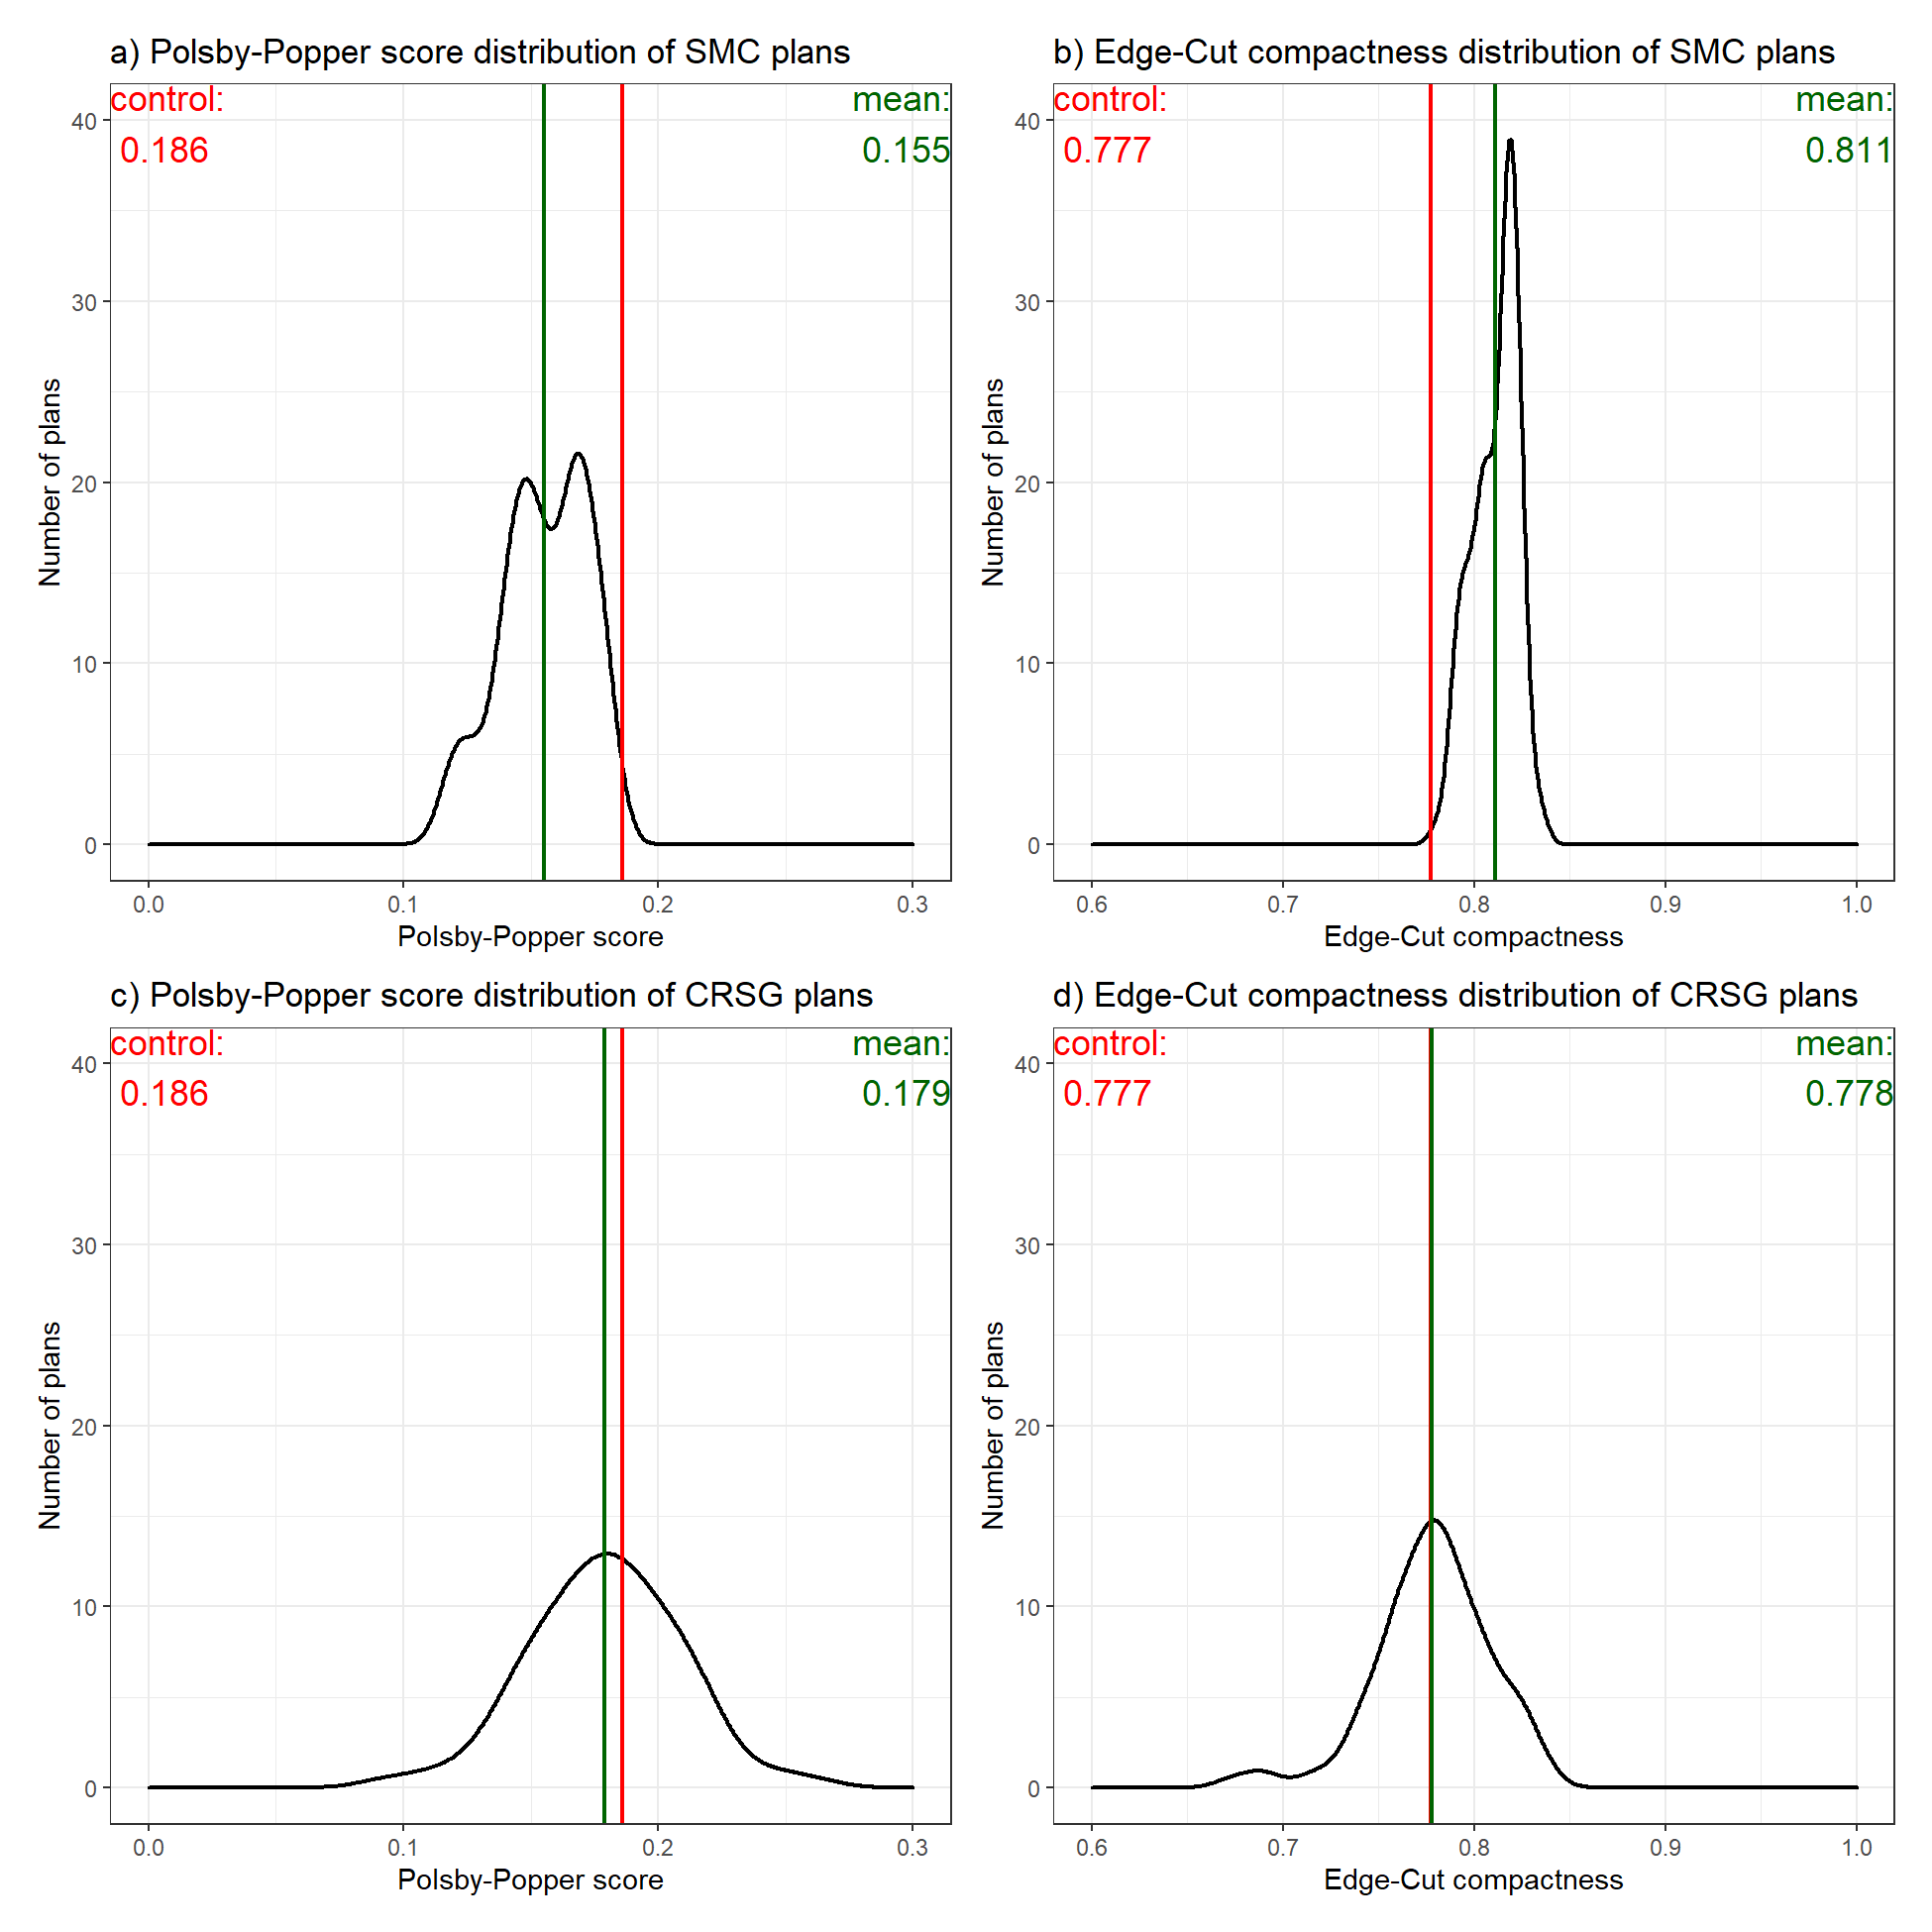
\includegraphics[width=\textwidth]{img/compact.density.png}
    \label{fig:compact.density}
    \raggedright
    \figurenote{The first column of plots shows the \hyperref[sec:polsbypopper]{Polsby-Popper} score distribution; the second column shows the \hyperref[sec:edgecut]{Edge-Cut compactness} distribution. The first row corresponds to the plans generated by SMC; the second row corresponds to CRSG. The dashed red lines indicate the measure value for the existing districts; the solid blue lines indicate the mean value of the distribution.}
\end{figure}

Figure \ref{fig:compact.density} visualizes the distribution of two different compactness scores amongst plans generated by both SMC and CRSG. Subfigure
\begin{seriate} 
    \item shows the distribution of the \hyperref[sec:polsbypopper]{Polsby-Popper scores} of the 100 SMC plans, subfigure
    \item shows the distribution of the \hyperref[sec:edgecut]{Edge-Cut compactness measure} of the same 100 SMC plans, and subfigures
    \item and 
    \item show the corresponding measure distributions for the plans generated by CRSG. 
\end{seriate}
The dashed red lines indicate the value of the measure for the existing district map, and the solid blue lines indicate the mean value of the distribution. 

\subsection{Partisan Fairness}

\subsubsection{Seats-Votes Curves}

\begin{figure}[h]
    \caption{Seats-Votes Curves for SMC- and CRSG-Generated Maps and Existing Map}
    \begin{subfigure}[b]{0.45\textwidth}
        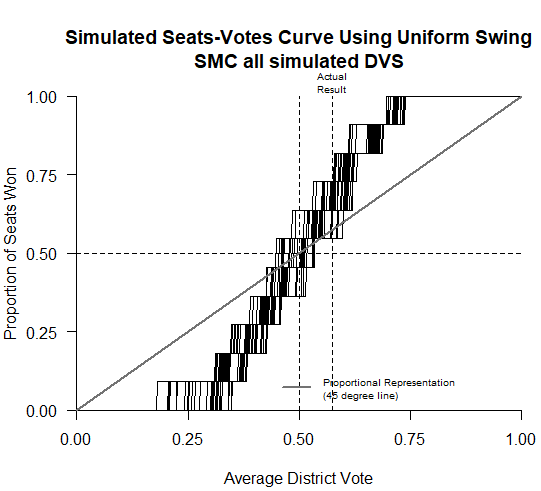
\includegraphics[width=\textwidth]{img/sv.smc.png}
        \caption{SMC Curve}
        \label{fig:sv.smc}
    \end{subfigure}
    \hfill
    \begin{subfigure}[b]{0.45\textwidth}
        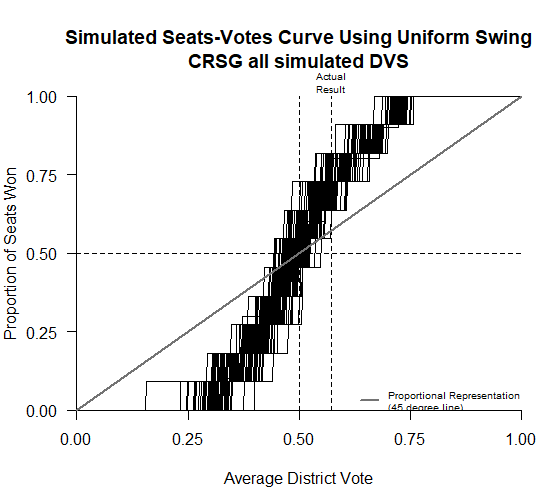
\includegraphics[width=\textwidth]{img/sv.crsg.png}
        \caption{CRSG Curve}
        \label{fig:sv.crsg}
    \end{subfigure}
    \vskip\baselineskip
    %\hfill
    \begin{subfigure}[b]{0.45\textwidth}
        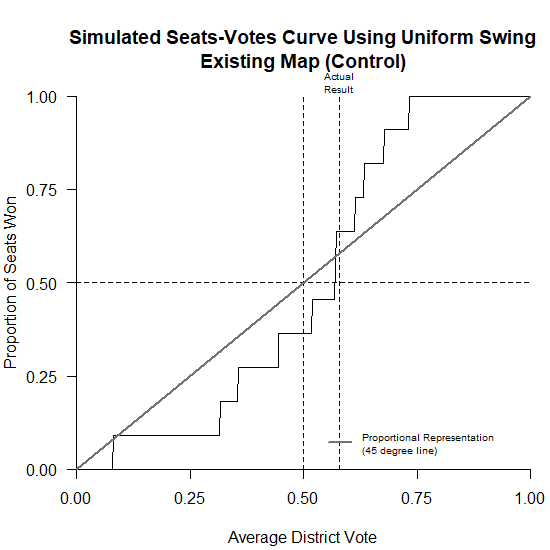
\includegraphics[width=\textwidth]{img/sv.control.png}
        \caption{Control Curve}
        \label{fig:sv.control}
    \end{subfigure}
    \label{fig:sv}
    \raggedright
    \figurenote{Each plot shows the relationship between average proportion of Democratic vote share by district and the proportion of Democratic seats. Subfigure \ref{fig:sv.smc} illustrates this relationship for the 100 plans generated by SMC, subfigure \ref{fig:sv.crsg} for CRSG, and subfigure \ref{fig:sv.control} is for the existing map.}
\end{figure}

Figure \ref{fig:sv} shows the seats-votes curves \parencite{katz2020} for the 2018 General Election under the redistricting plans generated by both algorithms and the existing map, the control. For each plot, the x-axis plots the average of the proportion of votes won by Democrats in each district, the average DVS. The y-axis plots the proportion of seats won by Democrats in the delegation. Both subfigures \ref{fig:sv.smc} and \ref{fig:sv.crsg} have once curve for each redistricting plan (each plot has 100 curves). The seats-votes curve for the real 2018 districts is provided for reference in subfigure \ref{fig:sv.control}.

\subsubsection{Single-Valued Partisan Fairness Measures}

Figure \ref{fig:fair.density} illustrates the distributions of various fairness measures within the plans generated by SMC and CRSG. Columns of plots correspond to different measures, and rows of plots correspond to different algorithms. The dashed red and solid blue vertical lines indicate the control value and mean distribution value, respectively. 

\begin{landscape}
    \begin{figure}[h]
        \caption{Distributions of Partisan Fairness Measures for SMC- and CRSG-Generated Maps}
        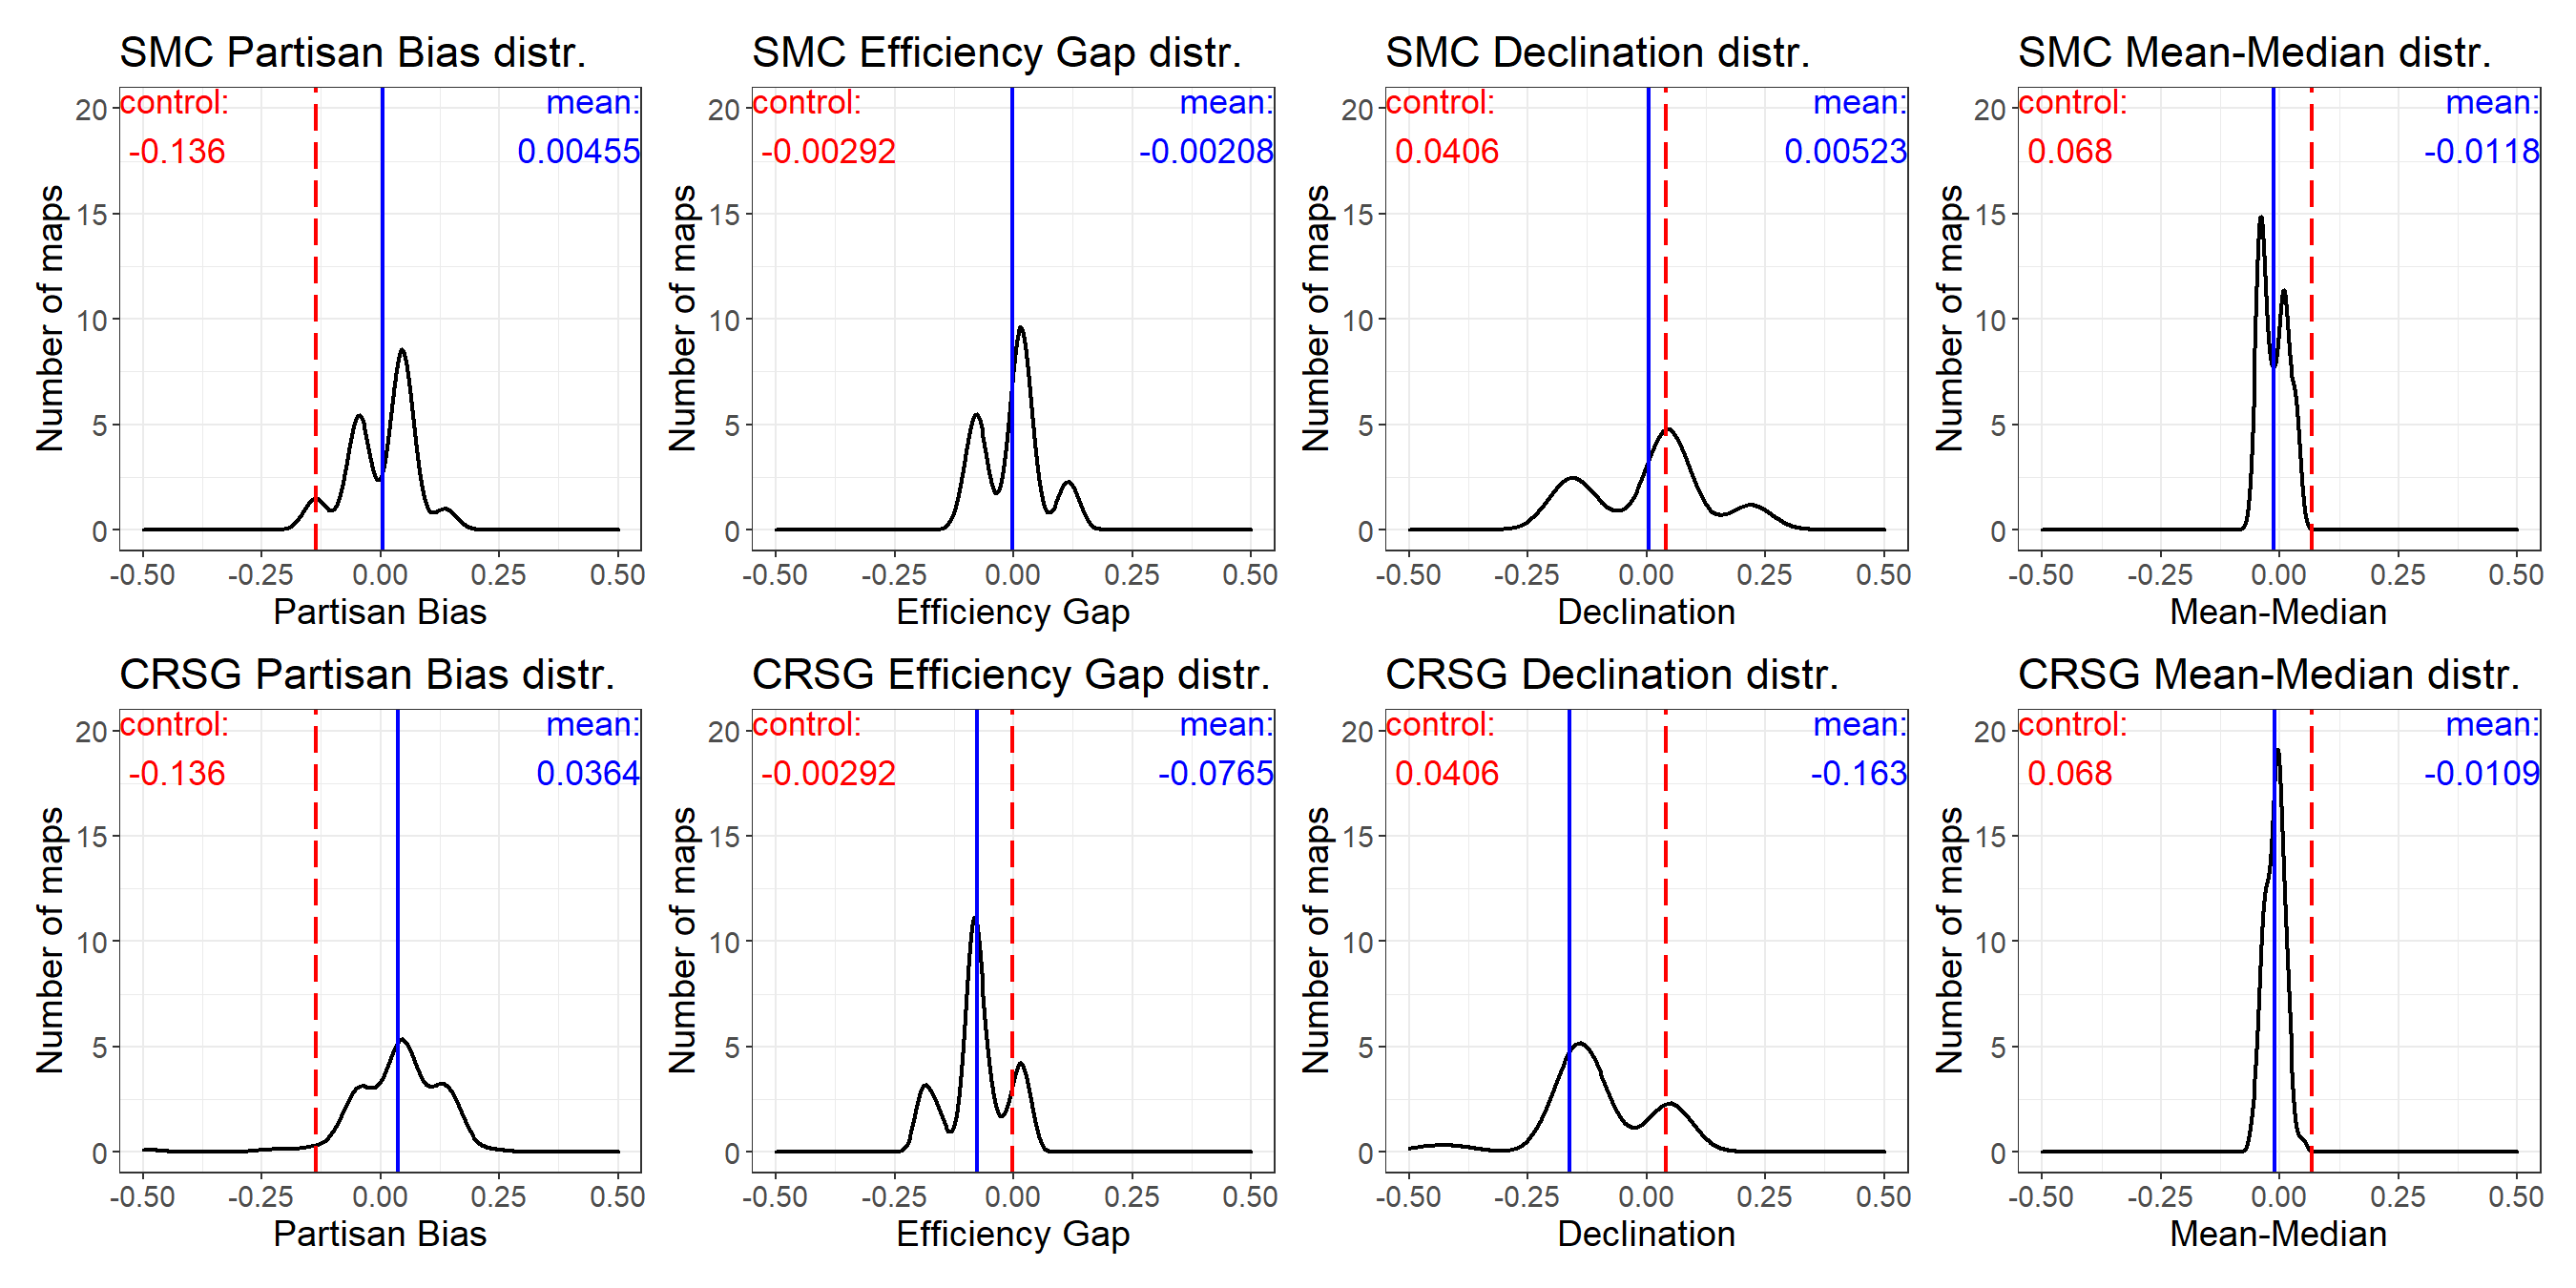
\includegraphics{img/fair.density.png}
        \label{fig:fair.density}
        \raggedright
        \figurenote{The columns of plots illustrate the distributions of \hyperref[sec:bias]{partisan bias}, the \hyperref[sec:effgap]{efficiency gap}, \hyperref[sec:declination]{declination}, and the \hyperref[sec:meanmed]{mean-median difference}, respectively. The first row of plots corresponds to SMC plans, the second to CRSG plans. The dashed red lines indicate the corresponding value of the measure in the existing plan; the solid blue lines indicate the mean value of the distribution.}
    \end{figure}
\end{landscape}